\section{Eiffage table plan}
\label{eiffageTablePlan}

%TODO Afficher des plans
\begin{figure}[h]
    \centering
    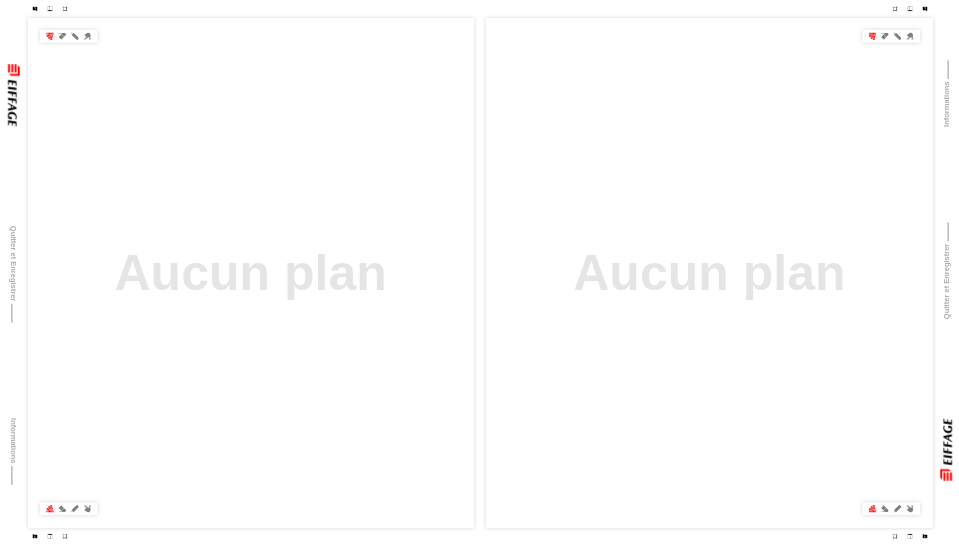
\includegraphics[scale=0.5]{img/table-plan-capture.png}
    \caption{Capture d'écran de l'application Table Plan}
\end{figure}

Dans le trio d'applications de la nouvelle salle cockpit d'Eiffage, l'application d'édition de plan m'a été accordée en partie.
L'objectif de cette application est d'afficher et de permettre la manipulation de plans (au format PDF) issus de  l'espace réseau d'Eiffage.
Cette application est affichée sur un écran intégré dans une table faite sur mesures permettant l'interaction de plusieurs personnes au même moment.

Le cahier des charges de cette application est le suivant :
\begin{itemize}
    \item Charger et afficher des plans depuis le réseau d'Eiffage
    \item Permettre aux utilisateurs de manipuler les plans affichés
    \item Permettre aux utilisateurs d'annoter les plans affichés et d'enregistrer ces annotations pour les transmettre à l'architecte
    \item Utiliser un design compatible avec l'affichage sur une table tactile où plusieurs personnes sont assises autour d'un écran affichant l'application.
\end{itemize}

\subsection{Application existante}
\label{eiffageTablePlanApplicationExistante}

Cette application était la plus avancée des trois lors du début du projet.
L'équipe précédente avait beaucoup travaillé sur l'affichage des PDF .

En effet, les PDF d’ Eiffage sont très lourds et demandent un affichage particulier.
L'équipe ayant travaillé sur ce projet a donc beaucoup réfléchi à la technologie à utiliser pour afficher les PDF sans ralentissement.
Ils ont donc opté pour une approche orientée Web avec un chargement, non pas du PDF en lui même, mais d'une image de ce PDF rendue à l'aide de ImageMagick.
Ils ont alors utilisé PixiJs, une librairie 2D pour WebGL, pour afficher l'image du PDF et permettre l'annotation.

Le plus gros de l'application, l'édition de plan était déjà codée et j'ai donc eu l'objectif de créer l'interface pour qu'elle reflète les créations du designer.
Mais aussi que l'application soit utilisable en collaboration et donc autour d'une table.

En revanche, l'ancienne application n'utilisait pas les WebComponents et j'ai dû m'adapter pour reformer le code présent.
De plus, le développeur me précédent, n'avait pas du tout les mêmes habitudes de développement et la même structure que moi et j'ai donc eu une longue phase d'analyse pour comprendre le rôle de chaque élément.

\subsection{Technologie}
\label{eiffageTablePlanTechnologie}

Les technologies utilisées dans le cadre de ce projet sont les mêmes que les autres applications de ce type créent par LTBL.
On y retrouve Electron pour l'affichage de l'application et les WebComponents pour la structure interne.

\subsection{Structure}
\label{eiffageTablePlanStructure}

L'application se divise alors en de multiples WebComponents chacun ayant un rôle spécifique.

\begin{figure}[h]
    \centering
    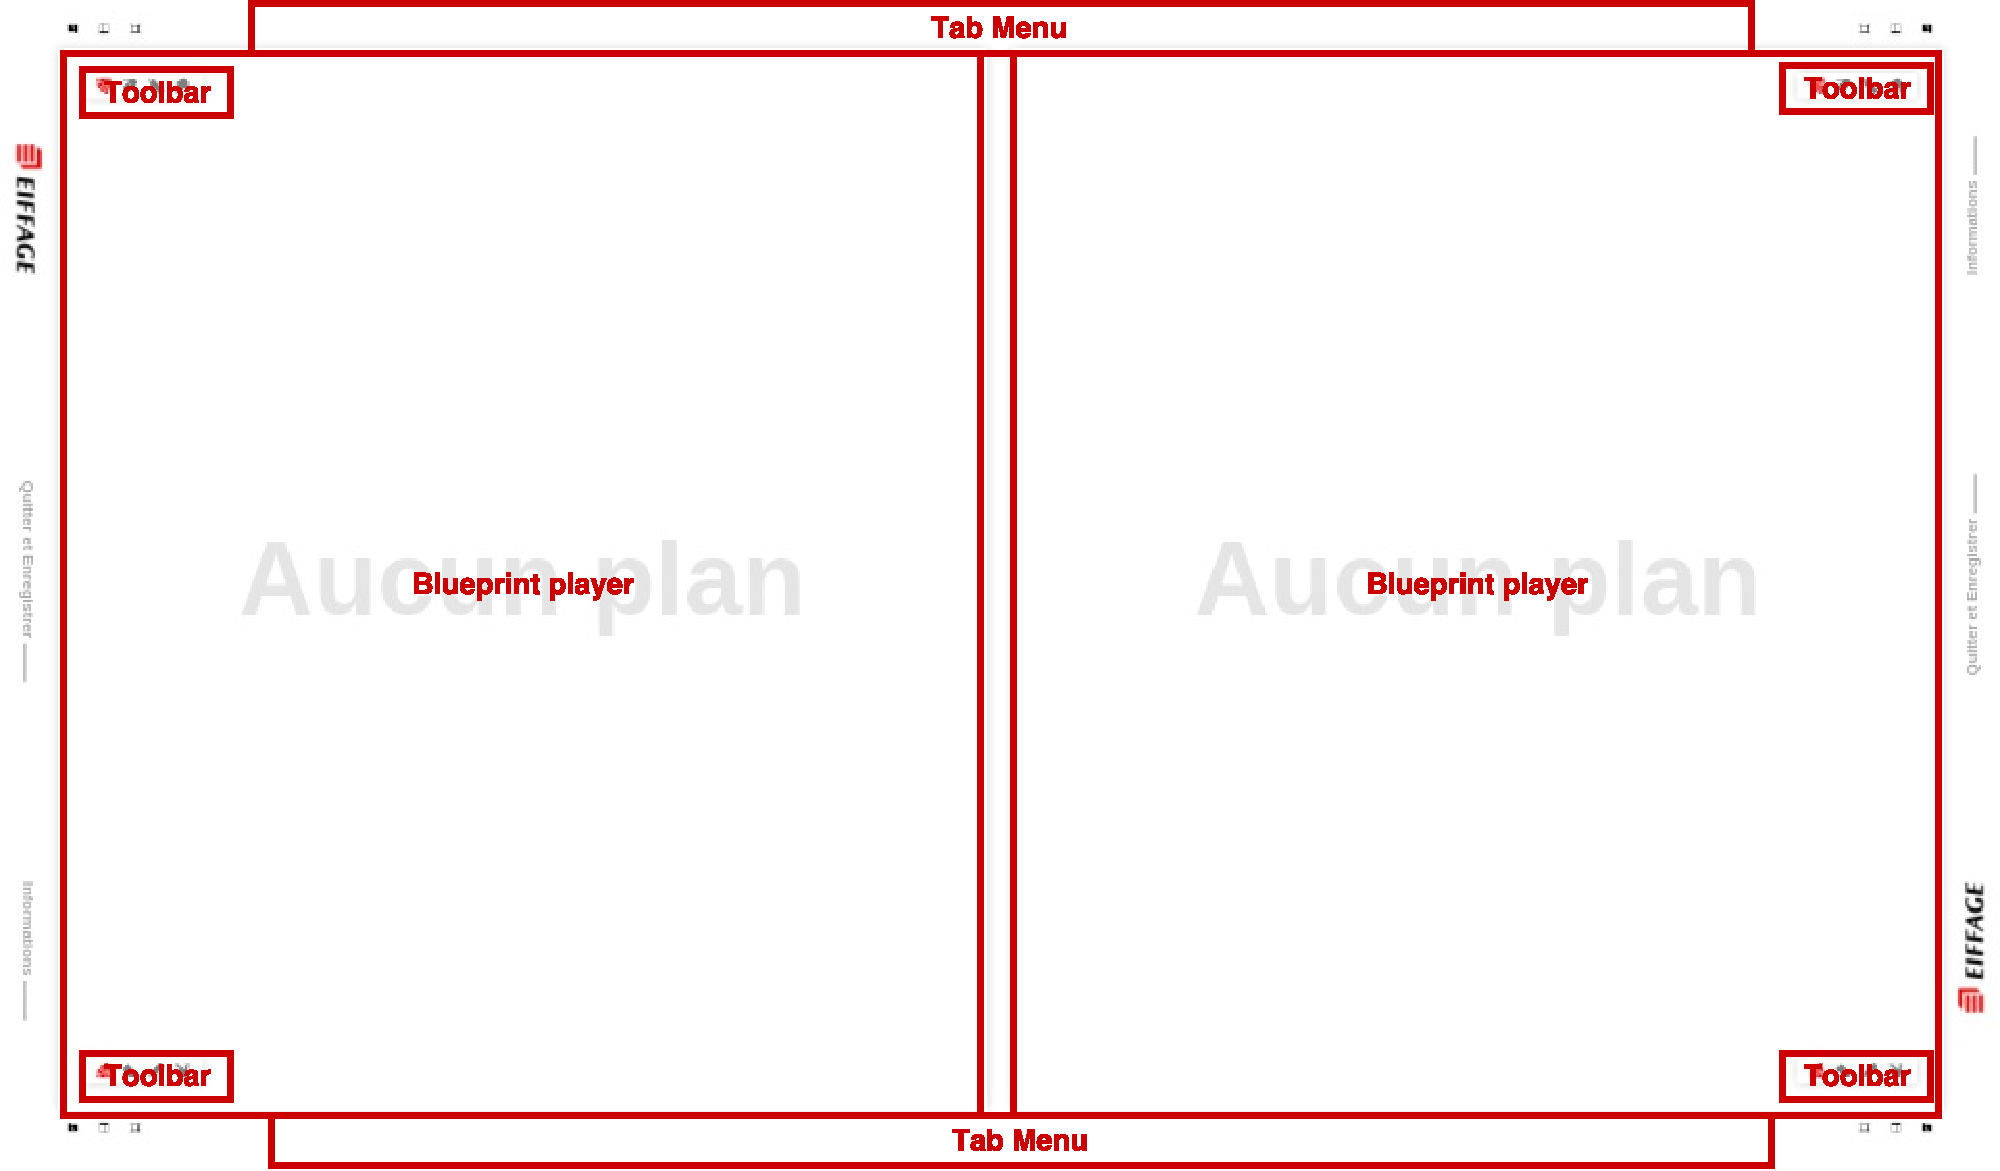
\includegraphics[scale=0.5]{img/table-plan-structure.pdf}
    \caption{Structure de l'application Table Plan}
\end{figure}

On retrouve alors les composants suivants

\paragraph{Blueprint player} Un component en charge d'afficher et d'annoter un plan dans notre cas.
Ce component était déjà, en grande partie, conçu quand j'ai débuté le développement de l'interface.
Anisi, je n'ai eu qu'à l'intégrer dans l'application finale.

\paragraph{Tab menu} Le menu composé de différents onglets.
Chaque onglet représente un plan ouvert qui peut être affiché.
Ce component est présent en 2 exemplaires dont un retourné sur le haut de l'application destiné aux utilisateurs présents de l'autre côté de la table.
J'ai synchronisé l'état de ces deux components avec un système de Store (\emph{cf} partie\ref{eiffageTablePlanStores})

\paragraph{Toolbar} Un composant affichant divers boutons permettant de choisir l'outil à utiliser dans sur le plan affiché.
Ce component est présent en 4 exemplaires dans l'application et doit donc être synchronisé avec ses voisins.
J'ai aussi utilisé le système de store pour synchroniser les états des barres d'outils et des éditeurs de plans (\texttt{Blueprint Player}).

\bigskip

Dans cette application, j'ai aussi utilisé le component \texttt{Media reader} du projet précédent pour offrir une interface unifiée sur toutes les applications développées pour Eiffage.
Je l'ai ajouté par le biais des submodules Git et de quelques petits ajustements dans le code de base de l'explorateur.

\subsection{Style}
\label{eiffageTablePlanStyle}

L'un des points majeurs de cette mission fut le style de l'application.
En effet, on est loin d'une application standard exécutée sur un bureau.
On remarque que l'utilisation faite de cette application nécessite une mise en place particulière des éléments de l'interface.

On remarque notamment que les barres d'outils sont présentes aux 4 coins de l'interface toutes dirigés vers l'extérieur de l'application pour permettre an'importe quel collaborateur autour de la table d'interagir avec les plans.
Cela a demandé la mise en place d'une synchronisation des barres d'outils au niveau de l'application et l'utilisation de propriétés CSS de transformations a des fins bien plus ergonomiques qu'esthétiques.

\bigskip

On remarque aussi que la barre des onglets ouverts est aussi inversée sur la partie supérieure de l'application.
Cela a demandé une modification au niveau du code lui-même, car je ne pouvais pas me contenter d'effectuer un miroir sur l'élément (ce que j'ai fait pour les barres d'outils).
La raison de cette spécificité est la présence de texte.
Mettre un effet de miroir sur un texte le rend complètement illisible (contrairement à une icône) et j'ai effectué une rotation au lieu de faire un miroir.
Mais cela posé d'autres problèmes puisque la droite et la gauche était inverse sur chacun des éléments.
J'ai donc modifié le code source du composant de la barre d'onglets pour qu'elle inverse toutes les commandes dans certains cas.

\subsection{Stockage de données}
\label{eiffageTablePlanStores}

Par son style particulier et la dimension collaborative de la table, de nombreux éléments de l'interface doivent être synchronisés.
Par exemple, il faut synchroniser l'état des barres tout'ils pour qu'elles affichent en tout temps le bon outil en cours d'utilisation même si cet outil est changé depuis un élément extérieur comme une autre barre d'outils.

J'ai, dans un premier temps, imaginé un système inclus dans les components permettant de les lier directement pour qu'ils s'informent entre eux lors d'un changement d'état d'un côté.

\begin{figure}[h]
    \centering
    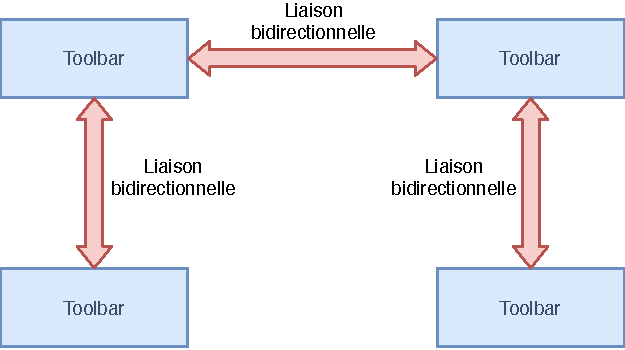
\includegraphics[scale=1]{img/premiere-synchro.pdf}
    \caption{Premier système de synchronisation utilisé dans le cas des barres d'outils de l'application}
\end{figure}

Cela fonctionnait, mais je me suis vite heurté à la rigidité de ce système et à la complexité d'étendre les fonctionnalités de ce système à l'application entière.
J'ai donc puisé dans mes connaissances et me suis inspiré des solutions trouvées dans des librairies comme \emph{Vuex} pour concevoir les Stores.

Un store est une classe Singleton\footnote{Une classe qui ne peut être instanciée qu'une seule fois et accessible par tout le programme}  qui va stocker un état particulier.
Cette classe est observable et peut donc informer les éléments de l'interface qui lui sont abonnés des changements apportés à l'état du store.
Ce système permet de centraliser la gestion des informations à l'échelle de l'application sans pour autant rendre les components dépendants les uns des autres.
De plus, ce système permet une grande flexibilité, car on peut modifier l'état à n'importe quel endroit de l'interface.
Ces changements seront alors répercutés sur l'ensemble de l'application automatiquement et dynamiquement.

\begin{figure}[h]
    \centering
    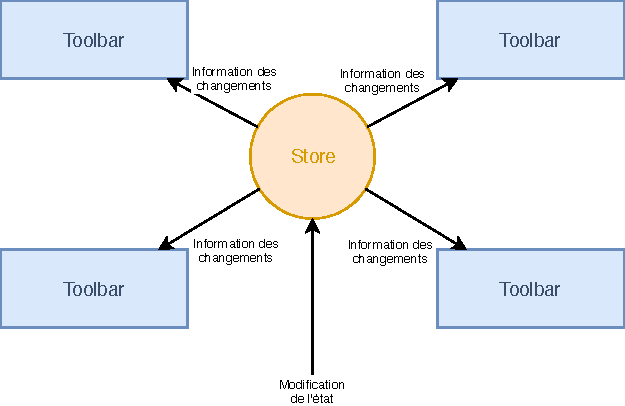
\includegraphics[scale=1.5]{img/store.pdf}
    \caption{Le fonctionnement du store dans le cadre de la gestion des barres d'outils}
\end{figure}

J'ai alors réutilisé ce système dans la gestion des plans ouverts et en cours de conversion (\emph{cf} partie \ref{eiffageTablePlanConversion}) sur Tableplan.
Mais aussi dans les autres applications que j'ai été amené à développer à la suite de celle-ci.

\clearpage

\subsection{Conversion}
\label{eiffageTablePlanConversion}

Les plans d'Eiffage étant très lourds, ils sont impossibles à ouvrir tel quel dans l'application.
Il faut donc utiliser un logiciel de conversion pour rendre les PDF sous forme d'image.

Les PDF de plans d'Eiffage étant des plans vectoriels\footnote{Une image vectorielle est une image dont on ne spécifie pas la couleur de chaque pixel, mais on spécifie une suite d'instruction permettant de calculer l'image finale. Les fichiers PDF, AI et SVG sont des exemples de fichiers vectoriels} Ils nécessitent un calcul préalable pour les afficher.
Pour résoudre le problème de lourdeur des fichiers, j'ai mis en place un système de conversion automatique des plans.

\bigskip

Dès qu'un fichier PDF est ouvert, on vérifie dans un dossier de cache s'il n'est pas déjà converti.
S’ il l'est, on ouvre simplement la conversion précédente.
S'il ne l'est pas, on lance une conversion.
On informa alors l'utilisateur de la conversion en cours et on attend la fin de cette conversion avant d'ouvrir le fichier converti.

\begin{figure}[h]
    \centering
    
\includegraphics[scale=0.3]{img/image-magick.png}
    \hspace{5cm}
    
\includegraphics[scale=0.13]{img/ghostscript.png}
    \caption{Les logis de ImageMagick (à gauche) et GhostScript (à droite)}
\end{figure}

La conversion est effectuée avec ImageMagick, un logiciel de manipulation d'images très performant, et de GhostScript, un logiciel permettant de rendre des fichiers PDF avec ImageMagick.

Pour permettre un rendu optimal dans toutes les circonstances, nous avons choisi de rendre les plans en 4K et de les afficher dans une fenêtre 4 fois supérieure à leur taille pour avoir un trait d'annotation fin bien défini.

\subsection{Conclusion}
\label{eiffageTablePlanConclusion}

Ce projet fut pour moi l'occasion d'expérimenter plus en profondeur les stockages des données au sein d'une application basée sur des composants.
Ce fut aussi une bonne expérience de travail en équipe, car je n'ai développé que l'interface qui entourait un système d'affichage et d'annotation de plans développé par le reste de l'équipe.
